\label{chap:openmp}

\section{Introduction}
Transformations in Polly create loops that are executed in parallel, as if the user would have
added some OpenMP pragmas. To achieve this, code generation needs to emit code that calls OpenMP
library functions to be executed in parallel. The GNU OpenMP Library(libgomp) is used for this purpose. The
dependency analysis module of Polly automatically detects parallel loops(SCoPs) and are given to OpenMP
code generation module. Here we generate the required libgomp library calls. The generated code is similar
to the one generated if the user have added OpenMP pragmas\cite{parfor}. The following sections explain the steps
taken towards generating the OpenMP code. The generated code is in LLVM IR format.

\section{Generating OpenMP Library Calls}

Typically when a user want to run a particular section of the code in parallel he/she annotate the code with
OpenMP pragmas. The compiler will then convert this pragmas into the corresponding library calls. In Polly the
approach taken is to generate these calls automatically when a loop is detected as parallel.

Consider the for loop in ~\ref{fig:openmp1} to have a basic understanding about what is to be done.
This is detected as a parallel and given for OpenMP code generation. Here the following
sequence of GOMP library calls with proper arguments and return types(signature) has to be generated in
LLVM IR format.

\begin{figure}
\begin{lstlisting}
  for (int i = 0; i <= N; i++)
    A[i] = 1 ;
\end{lstlisting}
	\caption{An example}
	\label{fig:openmp1}
\end{figure}

\begin{itemize}
\item GOMP\_parallel\_loop\_runtime\_start
\item subfunction
\item GOMP\_parallel\_end
\end{itemize}

\begin{figure}
  \label{fig:openmp_cfg}
  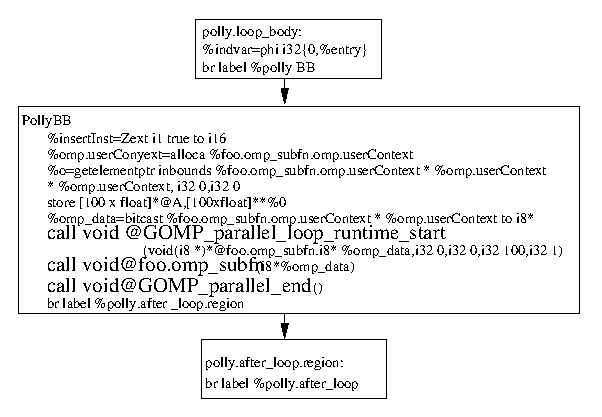
\includegraphics[width=1\textwidth]{images/ompcalls.eps}
  \caption{CFG showing sequence of OpenMP library calls}
\end{figure}

The control flow graph corresponding to the simple code in ~\ref{fig:openmp1} is shown in ~\ref{fig:openmp_cfg}
The code for body of the for loop is generated inside the subfunction which has the following GOMP library
calls to achieve the necessary parallelism.

\begin{itemize}
\item GOMP\_loop\_runtime\_next
\item GOMP\_loop\_end\_nowait
\end{itemize}

The signature and descriptions of each of the above functions can be found in in libgomp manual\cite{libgomp}.

\section{Support for inner loops}

So far OpenMP code created apply only for outermost loops, which is detected as SCoP. Next step is to do it for
inner loops. Due to dependency issues the outer loop is not detected as SCoP, but innerloop can be safely
parallelized as in the following example.

\begin{lstlisting}
  for (int i = 0; i < M; i++)
    for (int j = 0; j < N; j++)
      A[j] += M;
\end{lstlisting}

Those loops need the values of the surrounding induction variables and parameters in the OpenMP subfunction. We need
to pass the values of the outer induction variables in a structure to the subfunction. All the required variables
were already available in a datastructure used by Polly. We just needed to copy those into the body of the subfunction
so that it can refer those whenever needed.

\section{Adding OpenMP testcases}

<give more explanation>

\section{Dealing with memory references}

\begin{lstlisting}
#define N 10
  void foo() {
    float A[N];
    for (int i=0; i < N; i++)
      A[i] = 10;
    return;
}
\end{lstlisting}

Consider the above code segement. The 'for' loop will be detected as parallel by Polly and will be embedded in the
body of the OpenMP subfunction. But it accesses a non-global array 'A' and so accessing the same will not be possible inside
the subfunction. The approach for solving this issue is explained below.

\subsection{Adding memory references}

The base addresses of all memory references made by a statement is available in each statement instance. Prior to creating the body
of the subfunction we add all these base addresses are added into the same data structure where we stored the induction variables and parameters.
And then it is added to the subfunction structure.

\subsection{Extracting memory references}

Inside the body of the subfunction the base addresses are extracted from the subfunction structure and a new LLVM load instruction is created for each. The
new base addresses mapped to the old addresses so that any future references are made on the new addresses.

